\documentclass[12pt]{beamer}
\usetheme{Warsaw}
\usepackage[utf8]{inputenc}
\usepackage[english]{babel}
\usepackage{amsmath}
\usepackage{amsfonts}
\usepackage{amssymb}
\usepackage{graphicx}
%\author{Laura Tamayo Blanco}
\author[Laura Tamayo Blanco]{Laura Tamayo Blanco\\Tutor: MSc. Damian Valdés Santiago}

\title{Detección de metáforas en el discurso público cubano}
%\setbeamercovered{transparent} 
%\setbeamertemplate{navigation symbols}{} 
%\logo{} 
%\institute{} 
\date{14 de diciembre 2022} 
%\subject{} 
\begin{document}

\begin{frame}
\titlepage
\end{frame}

%\begin{frame}
%\tableofcontents
%\end{frame}
%Introducción
\begin{frame}{¿Qué es una metáfora?}
\begin{itemize}
\item Recurso del lenguaje.
\item Asocia dos conceptos que de forma literal no se verían juntos.
\item Permite entender la forma de pensar de la sociedad en un momento dado.
\end{itemize}
\end{frame}


\begin{frame}{CORESPUC}
Proyecto Nacional: Dinámicas sociales, políticas y económicas en el discurso público en Cuba de principios del siglo XXI: estudios CORESPUC. \\
\end{frame}

\begin{frame}{Objetivo}
Implementar un algotitmo para la detección automática de la metáfora.
\end{frame}
%Estado del arte
\begin{frame}{Tipos de metáfora}
\begin{itemize}
\item Metáfora conceptual.
\item Metáfora lingüística.
\end{itemize}
\end{frame}

\begin{frame}{Metáfora conceptual}
Según grado de aceptación:
\begin{itemize}
\item Metáfora novedosa: \textit{debutó en Facebook}.
\item Metáfora convencional:  \textit{perder el tiempo}.
\item Metáfora muerta.
\end{itemize}
Según dominio de mapeo:
\begin{itemize}
\item Metáforas estructurales: \textit{palabras vacías}.
\item Metáforas de orientación:  \textit{caer en el alcoholismo}.
\item Metáforas ontológicas: \textit{la inflación avanza}.
\end{itemize}
\end{frame}

\begin{frame}{Metáfora lingüísticas}
Según cantidad de palabras:
\begin{itemize}
\item  Metáforas léxicas:
\begin{enumerate}
\item Tipo I o Nominales: \textit{como tiburón viejo}.
\item Tipo II o Sujeto -Verbo - Objeto (SVO): \textit{devoró el libro}.
\item Tipo III o Adjetivo -Sustantivo (AN): \textit{energía verde}.
\item Tipo IV o Adverbio-Verbo (AV): \textit{hablar fluidamente}.
\end{enumerate}
\item Metáforas multi-palabra.
\item Metáforas extendidas.
\end{itemize}
\end{frame}

\begin{frame}{Trabajos relacionados}
\begin{itemize}
\item En 2014, Tsvetkov[2014] creó un corpus con metáforas léxicas de tipo II y III.
\item En 2018, Opolka[2018] utilizaron un modelo de redes neuronales sobre el corpus VUA.
\item  En 2021, Sánchez[2021] construyó un corpus en español (CoMeta).
\end{itemize}
\end{frame}
%Marco teórico e implementación
\begin{frame}{Word embeddings}
Los \textit{word embeddings} son un conjunto de técnicas, que buscan representar el texto con vectores de números reales de manera tal que si dos vectores son cercanos es posible decir que tienen significados similares.
\end{frame}
\begin{frame}{Redes neuronales}
\begin{itemize}
\item Un tipo de modelo que se utiliza para realizar aprendizaje supervisado.
\item Conjunto de neuronas organizadas por capas, cada neurona posee una entrada y una salida mediante conexiones con otras neuronas.
\item Dichas conexiones tienen pesos propios, de ahí que una red neuronal sea comparada con un grafo dirigido ponderado.
\end{itemize}
\end{frame}

\begin{frame}{Forma del corpus}
\begin{center}
 ADJETIVO SUSTANTIVO ETIQUETA
\end{center}
Originalmente: 200 pares (100 metáforas, 100 literales).\\
Tras la expansión: 1462 pares (762 metáforas, 700 literales).
\end{frame}

\begin{frame}{LSTM}
\begin{figure}[htb]\label{Fig:lstm_mod}
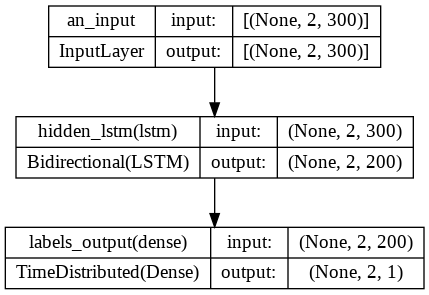
\includegraphics[scale= 0.6]{Graphics/lstm_metaphor_model.png}
\caption{Arquitectura del modelo LSTM.}
\end{figure}
\end{frame}
\begin{frame}{GRU}
\begin{figure}[htb]\label{Fig:gru_mod}
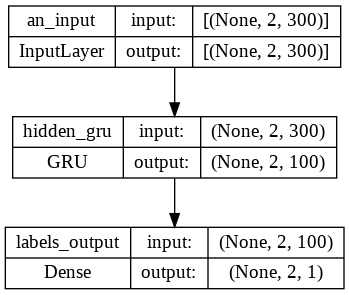
\includegraphics[scale= 0.6]{Graphics/gru_metaphor_model.png}
\caption{Arquitectura del modelo GRU.}
\end{figure}
\end{frame}


\begin{frame}{Resultados LSTM}
\begin{table}[hbt]
\centering
\begin{tabular}{c|c|c|c}
Épocas & F1 & Precisión & Recobrado\\
\hline
5 & 0.7148 & 0.5767 & 0.9552\\
\hline
7 & 0.7176 & 0.5788 & 0.9607\\
\hline
10 & 0.7175 & 0.5782 & 0.9607\\
\hline
\end{tabular}
\caption{Experimentos con el modelo LSTM. \label{Tabla:1}}
\end{table}
\end{frame}
\begin{frame}{Resultados GRU}
\begin{table}[htb]%
\centering
\begin{tabular}{c|c|c|c}
Épocas & F1 & Precisión & Recobrado\\
\hline
5 & 0.6304 & 0.4663 & 0.9833\\
\hline
7 & 0.5460 & 0.3912 & 0. 9264\\
\hline
10 & 0.5959 & 0.5730 & 0.6387\\
\hline
\end{tabular}
\caption{Experimentos con el modelo GRU \label{Tabla:2}}%
\end{table}
\end{frame}
\begin{frame}{Comparación con CoMeta}
\begin{table}[htb]%
\centering
\begin{tabular}{c|c|c|c|c}
Modelo & Épocas & F1 & Precisión & Recobrado\\
\hline
CoMeta & 10 & 0.3346 & 0.2324 & 0.5972\\
\hline
LSTM & 10 & 0.2684 & 0.1618 & 0.8435\\
\hline
GRU & 10 & 0.2171 & 0.1580 & 0.3469\\
\hline
\end{tabular}
\caption{Comparaciones con el estado del arte de CoMeta. \label{Tabla:3}}%
\end{table}
\end{frame}

\begin{frame}{Construcción del corpus del periódico Vanguardia}
\begin{itemize}
\item Se utilizó el modelo LSTM descrito previamente.
\item Los datos en español se obtuvieron del periódico Vanguardia, de la provincia Villa Clara.
\end{itemize}
\end{frame}
\begin{frame}{Construcción del corpus del periódico Vanguardia}
\begin{itemize}
\item Se extrajeron los pares adjetivo sustantivo de los textos.
\item Utilizando traducción automática se llevaron al inglés.
\item Una vez traducidos se pasan al modelo. 
\end{itemize}
\end{frame}
\begin{frame}{Ejemplos}
\begin{figure}[htb]\label{Fig:good}
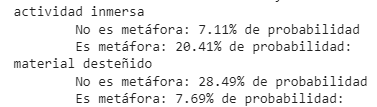
\includegraphics[scale= 1.0]{Graphics/good_example.png}
\caption{Ejemplos de resultados correctos.}
\end{figure}
\end{frame}
\begin{frame}{Ejemplos}
\begin{figure}[htb]\label{Fig:good}
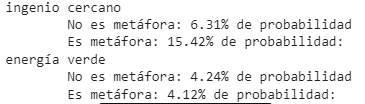
\includegraphics[scale= 1.0]{Graphics/bad_example.png}
\caption{Ejemplos de resultados incorrectos.}
\end{figure}
\end{frame}
\begin{frame}{Conclusiones}
\begin{itemize}
\item El modelo entrenado puede ser utilizado en un software para apoyar a los especialistas del lenguaje.
\item De los modelos propuestos el que mejores resultados obtuvo fue
el LSTM entrenado por 10 épocas.
\item Se acercó a las métricas del estado del arte.
\end{itemize}
\end{frame}
\begin{frame}{Recomendaciones}
\begin{itemize}
\item Determinar, con la ayuda de un lingüista, qué porciento de las etiquetas colocadas en el corpus es correcto .
\item Experimentar qué resultados se obtienen con otros \textit{word embeddings}.
\item Probar otras configuraciones de parámetros de los modelos presentados.
\end{itemize}
\end{frame}
\begin{frame}
\titlepage
\end{frame}

\begin{frame}{Preguntas del oponente}
\textbf{Uno de los objetivos del trabajo es construir un corpus utilizando datos del periodíco Vanguardia. ¿Cuáles fueron los resultados obtenidos al aplicar el modelo a los pares adjetivo-sustantivo extraídos de este periódico?}
\begin{table}[htb]%
\centering
\begin{tabular}{c|c|c|c}
Total & Pérdida & Metáforas & No Metáforas \\
\hline
9186 & 382 & 2435 & 6369 \\
\hline
$100 \%$ & $4.16 \%$ & $26.5 \%$ & $69.34 \%$ \\
\hline
\end{tabular}
\caption{Estadísticas del corpus. \label{Tabla:3}}%
\end{table}
\end{frame}
\begin{frame}{Preguntas del oponente}
\textbf{Como se expresa en el documento, existen múltiples tipos de metáforas. ¿Por qué se decidió utlizar solo metáforas linguísticas de Tipo III para el trabajo?}\\
En un estudio realizado en el 2013 por Gandy y col\footnote{  Lisa Gandy, Nadji Allan, Mark Atallah, Ophir Frieder, Newton Howard, Sergey Kanareykin, Moshe Koppel, Mark Last, Yair Neuman, y Shlomo Argamon. 2013. Automatic identification of conceptual metaphors with limited knowledge. En Proc. of the Twenty-Seventh AAAI Conference on Artificial Intelligence, páginas 328–334.} se plantea que el $24\%$ de las metáforas son basadas en adjetivos, de ahí que tengan relevancia lingüística.\\
Una de las formas más sencillas de embellecer un texto es añadir adjetivos, por lo que es posible encontrar muchas instancias de estos pares en textos.
\end{frame}
\end{document}
